\subsection{Implementation details}
\label{app:impl}
\textbf{Standardization.} Per benchmark, with training-row mean and standard deviation (observed cells only). Errors are always reported on the standardized scale (``MSE'') and, where stated, in score points; $R^2=1-\mathrm{MSE}/\mathrm{MSE}_{\textsc{mean}}$ with $\textsc{mean}$ the training-mean predictor on the same targets (its standardized MSE exceeds 1 because held-out models differ systematically from the history: 1.18 on random splits, 1.36 for new organisations, 3.25 for later releases, MTEB-main).
\textbf{Covariance.} Pairwise-complete correlation with $\ge5$ co-observed models per pair (else 0), eigenvalues clipped at $10^{-3}$ and rescaled to unit diagonal, then $\Sigma_\kappa=(1-\kappa)\hat C+\kappa I$ with $\kappa\in\{0,0.05,0.15,0.3,0.5\}$ chosen on an inner split (20\% of training rows as validation models; for each, a random half of its observed benchmarks (at most 10) plays $S$, the rest targets). The same inner split tunes FA rank $r\in\{1,2,3,4,6,8,12\}$ (restricted to $(N-r)^2>N+r$), ISVD rank/ridge, $K$ of \textsc{kNN} ($\{5,15,40\}$) and the \textsc{Hybrid} blend; \textsc{Gauss} was selected for the main pipeline \emph{because} it did best in that inner validation on MTEB-main.
\textbf{FA by EM} uses the missing-data E-step (per-row posterior over observed benchmarks), a small ridge on loadings (0.05), and a floor $\psi_j\ge0.02$ on unique variances; 300 iterations at most.
\textbf{Selectors.} \textsc{Greedy} is Eq.~\eqref{eq:greedy}; \textsc{Greedy-MI} maximizes $\mathrm{Var}(z_j\mid z_S)\,(\Sigma^{-1})_{jj}$ (the criterion of \citet{krause2008near} simplifies since $\mathrm{Var}(z_j\mid\text{all others})=1/(\Sigma^{-1})_{jj}$ does not depend on $S$); \textsc{$k$-medoids}: 5 $k$-means++-seeded restarts on $1-|\rho_{ij}|$, medoids are not nested in $k$; ``top-SNR'' ranks by factor-model communality over unique variance. ``Most-evaluated'' orders benchmarks by their number of training observations (ties by column order).
\textbf{Held-out targets.} $T_0$ is a random 30\% of the model's observed set (at least 2) with two draws per model for MTEB, four for HELM-22 (pool sizes: up to $\sim$195 on MTEB-main); for $N\le12$ the held-out target is each benchmark in turn. We evaluate $k\le0.7\,|C|-3$ roughly, capped at 40 (14 for HELM-22; $\min_i|C_i|-2$ for $N\le12$). A (model, target-draw) cell is used in a curve only if it is available for every $k$ of that curve.
\textbf{Aggregation.} For each (selector, predictor, $k$), values are averaged over random draws and cells, then over repeats/folds per model; the bootstrap resamples models (2000 replicates, seed fixed).

\subsection{Reproducibility}
\label{app:repro}
Code, the processed matrices' construction scripts, and a README with commands, seeds, timings and the script that generates every table and figure are in the supplementary archive.
\textbf{Pinned data:} MTEB results repository at commit \texttt{6dabbcc6} (CC0-1.0); Open LLM Leaderboard \texttt{contents} at \texttt{9c09a7ca} (no explicit license; 4,576 rows, we drop 80 flagged or duplicate model entries); HELM Lite release v1.13.0 (\texttt{core\_scenarios}, \texttt{mmlu}, \texttt{legalbench}, \texttt{wmt\_14} group files); LiveBench \texttt{model\_judgment} at \texttt{9704e5da} (a 7-task per-model summary; mean of per-question scores per model and task $\times100$). MTEB task types and languages come from the \texttt{mteb} package (v2.26.31; used only for task metadata, 958 of the 1,172 tasks matched; the others are typed by name). One MTEB score is the \texttt{main\_score} of the test split (validation or dev if no test split), averaged over language subsets; tasks with differing subset sets across models keep only the modal one; tasks with scores outside $[-100,100]$ (two hardware-speed tasks) are dropped.
\textbf{Compute:} CPU only (40 cores, 250 GB RAM, of which a few GB used). The full pipeline (\texttt{run\_everything.sh}: synthetic checks, all real-data runs, ablations, tables) took about 1.1 h wall-clock; the second stage ran up to $\sim$80 processes on the 40 cores, so the summed per-fold wall times (22.7 h) overstate CPU time; one MTEB-main random-split fold (tuning of 6 predictors + all selectors) takes $\approx$ 8 min on one core when the machine is not oversubscribed, the synthetic checks $\approx$ 5 min. Data: 3.4 GB for the cloned MTEB repository (extracted matrices: a few MB).

\subsection{Additional results}
\label{app:more}

\begin{figure}[h]
\centering
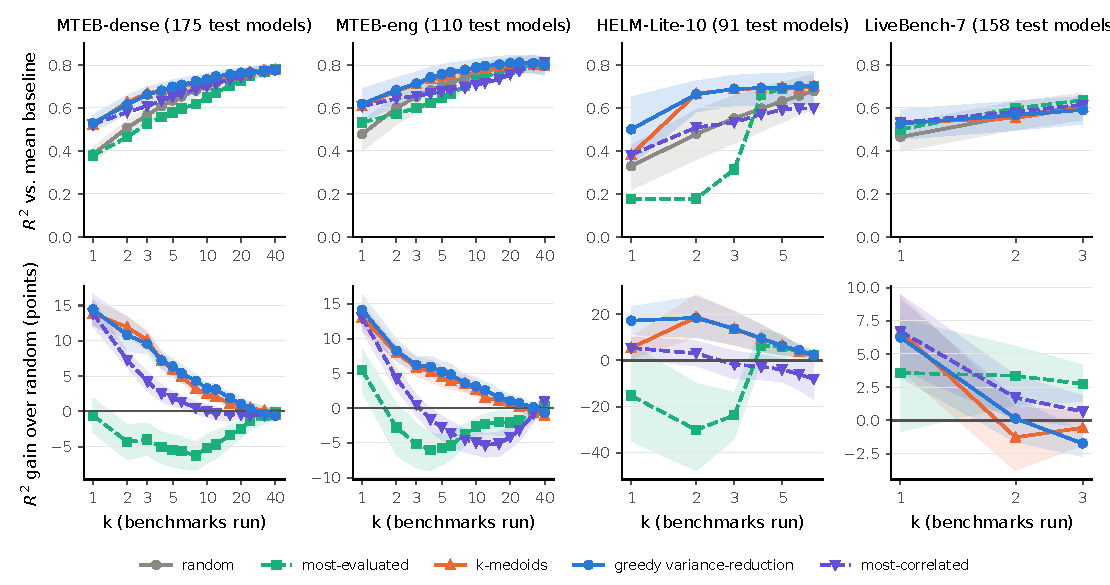
\includegraphics[width=\linewidth]{figs/curves_appendix.pdf}
\caption{As Fig.~\ref{fig:main} for the other matrices (random splits), with the most-correlated selector added. HELM-Lite-10 and LiveBench-7 have complete or nearly complete pools; the number of test models is the number of held-out models that have all budgets available.}
\label{fig:app_curves}
\end{figure}

\begin{table}[h]
\centering\small
\caption{Predictors on MTEB-main ($R^2$; random splits). 95\% CIs of $\pm$0.03--0.04 for each cell; paired differences in Appendix Table~\ref{tab:ci_pred}.}
\label{tab:pred}
\begin{tabular}{llccccc}\toprule
Selection & Predictor & $k{=}1$ & $k{=}5$ & $k{=}10$ & $k{=}20$ & $k{=}40$ \\\midrule
random & AvgShift & 0.40 & 0.55 & 0.58 & 0.60 & 0.61 \\
 & kNN & 0.45 & 0.67 & 0.74 & 0.77 & 0.78 \\
 & ISVD & 0.40 & 0.64 & 0.70 & 0.74 & 0.77 \\
 & FA & 0.38 & 0.65 & 0.71 & 0.76 & 0.78 \\
 & Gauss & 0.39 & 0.65 & 0.72 & 0.77 & 0.80 \\
 & Hybrid & 0.39 & 0.65 & 0.72 & 0.77 & 0.82 \\
\midrule
greedy variance-reduction & AvgShift & 0.53 & 0.58 & 0.59 & 0.59 & 0.60 \\
 & kNN & 0.60 & 0.70 & 0.75 & 0.77 & 0.78 \\
 & ISVD & 0.53 & 0.69 & 0.74 & 0.75 & 0.76 \\
 & FA & 0.54 & 0.71 & 0.75 & 0.77 & 0.79 \\
 & Gauss & 0.52 & 0.71 & 0.76 & 0.79 & 0.80 \\
 & Hybrid & 0.52 & 0.71 & 0.76 & 0.80 & 0.82 \\
\bottomrule
\end{tabular}

\end{table}

\begin{table}[h]
\centering\small
\caption{Standardized MSE under fixed held-out targets $T_0$ (this paper) vs.\ complement targets $C\setminus S$ (naive).}
\label{tab:bias}
\resizebox{\linewidth}{!}{\begin{tabular}{lllccc}\toprule
Dataset & Targets & Selector & small $k$ & mid $k$ & large $k$ \\\midrule
HELM-Lite-22 ($k{=}2,5,12$) & fixed $T_0$ & random & 0.67 & 0.54 & 0.42 \\
HELM-Lite-22 ($k{=}2,5,12$) & fixed $T_0$ & greedy variance-reduction & 0.63 & 0.48 & 0.41 \\
HELM-Lite-22 ($k{=}2,5,12$) & complement $C\!\setminus\!S$ & random & 0.66 & 0.48 & 0.42 \\
HELM-Lite-22 ($k{=}2,5,12$) & complement $C\!\setminus\!S$ & greedy variance-reduction & 0.61 & 0.42 & 0.27 \\
\midrule
MTEB-main ($k{=}2,10,40$) & fixed $T_0$ & random & 0.57 & 0.34 & 0.24 \\
MTEB-main ($k{=}2,10,40$) & fixed $T_0$ & greedy variance-reduction & 0.47 & 0.29 & 0.24 \\
MTEB-main ($k{=}2,10,40$) & complement $C\!\setminus\!S$ & random & 0.55 & 0.33 & 0.23 \\
MTEB-main ($k{=}2,10,40$) & complement $C\!\setminus\!S$ & greedy variance-reduction & 0.45 & 0.27 & 0.18 \\
\bottomrule
\end{tabular}
}
\end{table}


\begin{table}[h]
\centering\small
\caption{As Table~\ref{tab:main} for the other matrices.}
\label{tab:main_app}
\resizebox{\linewidth}{!}{\begin{tabular}{llcccc}\toprule
Dataset (split) & Selector & $k{=}1$ & $k{=}3$ & $k{=}5$ & $k{=}10$ \\\midrule
MTEB-dense (rand) & random & 0.38 \scriptsize[0.35,0.42] & 0.57 \scriptsize[0.53,0.60] & 0.63 \scriptsize[0.60,0.67] & 0.70 \scriptsize[0.67,0.73] \\
 & most-evaluated & 0.38 \scriptsize[0.34,0.42] & 0.53 \scriptsize[0.49,0.57] & 0.58 \scriptsize[0.54,0.61] & 0.65 \scriptsize[0.62,0.68] \\
 & k-medoids & 0.52 \scriptsize[0.48,0.56] & \textbf{0.67} \scriptsize[0.63,0.70] & 0.69 \scriptsize[0.66,0.72] & \textbf{0.73} \scriptsize[0.69,0.75] \\
 & greedy variance-reduction & \textbf{0.53} \scriptsize[0.49,0.57] & 0.66 \scriptsize[0.62,0.70] & \textbf{0.70} \scriptsize[0.66,0.73] & \textbf{0.73} \scriptsize[0.70,0.76] \\
\midrule
MTEB-eng (rand) & random & 0.48 \scriptsize[0.40,0.54] & 0.65 \scriptsize[0.58,0.71] & 0.70 \scriptsize[0.64,0.76] & 0.76 \scriptsize[0.70,0.80] \\
 & most-evaluated & 0.53 \scriptsize[0.45,0.60] & 0.60 \scriptsize[0.52,0.66] & 0.65 \scriptsize[0.58,0.70] & 0.73 \scriptsize[0.67,0.78] \\
 & k-medoids & 0.61 \scriptsize[0.53,0.67] & \textbf{0.71} \scriptsize[0.64,0.76] & 0.75 \scriptsize[0.69,0.79] & 0.78 \scriptsize[0.73,0.82] \\
 & greedy variance-reduction & \textbf{0.62} \scriptsize[0.53,0.69] & \textbf{0.71} \scriptsize[0.64,0.77] & \textbf{0.76} \scriptsize[0.70,0.80] & \textbf{0.79} \scriptsize[0.74,0.83] \\
\midrule
HELM-Lite-10 (rand) & random & 0.33 \scriptsize[0.22,0.43] & 0.55 \scriptsize[0.44,0.66] & 0.63 \scriptsize[0.53,0.72] & -- \\
 & most-evaluated & 0.18 \scriptsize[0.06,0.30] & 0.31 \scriptsize[0.23,0.39] & 0.69 \scriptsize[0.62,0.75] & -- \\
 & k-medoids & 0.38 \scriptsize[0.24,0.51] & \textbf{0.69} \scriptsize[0.61,0.75] & \textbf{0.70} \scriptsize[0.62,0.76] & -- \\
 & greedy variance-reduction & \textbf{0.50} \scriptsize[0.34,0.65] & \textbf{0.69} \scriptsize[0.61,0.75] & 0.69 \scriptsize[0.61,0.76] & -- \\
\bottomrule
\end{tabular}
}
\end{table}

\begin{table}[h]
\centering\scriptsize
\caption{Predictors on MTEB-main: paired difference $R^2_{\text{predictor}}-R^2_{\textsc{Gauss}}$ with 95\% bootstrap CI (positive = better than \textsc{Gauss}); the \textsc{Gauss} rows show its own $R^2$ [95\% CI].}
\label{tab:ci_pred}
{\tiny\setlength{\tabcolsep}{2pt}\begin{tabular}{llccccc}\toprule
Selection & Predictor & $k{=}1$ & $k{=}5$ & $k{=}10$ & $k{=}20$ & $k{=}40$ \\\midrule
random & AvgShift & +0.004 [+0.002,+0.006] & -0.099 [-0.113,-0.087] & -0.136 [-0.154,-0.121] & -0.168 [-0.188,-0.151] & -0.193 [-0.215,-0.173] \\
 & kNN & +0.053 [+0.030,+0.071] & +0.015 [-0.000,+0.029] & +0.018 [-0.001,+0.034] & -0.004 [-0.024,+0.014] & -0.021 [-0.042,-0.000] \\
 & ISVD & +0.003 [-0.009,+0.015] & -0.012 [-0.020,-0.005] & -0.020 [-0.028,-0.013] & -0.029 [-0.036,-0.022] & -0.036 [-0.045,-0.028] \\
 & FA & -0.009 [-0.019,+0.000] & -0.002 [-0.008,+0.004] & -0.007 [-0.013,-0.002] & -0.013 [-0.019,-0.007] & -0.021 [-0.031,-0.010] \\
 & Gauss & 0.394 [0.361,0.423] & 0.652 [0.618,0.684] & 0.720 [0.690,0.749] & 0.769 [0.743,0.793] & 0.802 [0.781,0.823] \\
 & Hybrid & -0.004 [-0.006,-0.002] & +0.001 [-0.001,+0.002] & +0.002 [+0.001,+0.004] & +0.005 [+0.003,+0.008] & +0.013 [+0.010,+0.018] \\
\midrule
greedy variance-reduction & AvgShift & +0.005 [+0.002,+0.008] & -0.128 [-0.146,-0.112] & -0.166 [-0.188,-0.146] & -0.199 [-0.233,-0.172] & -0.201 [-0.227,-0.177] \\
 & kNN & +0.075 [+0.047,+0.100] & -0.007 [-0.030,+0.014] & -0.010 [-0.034,+0.012] & -0.021 [-0.043,+0.001] & -0.020 [-0.043,+0.002] \\
 & ISVD & +0.006 [-0.004,+0.018] & -0.018 [-0.030,-0.008] & -0.023 [-0.032,-0.014] & -0.037 [-0.045,-0.030] & -0.036 [-0.044,-0.027] \\
 & FA & +0.018 [+0.006,+0.029] & +0.000 [-0.010,+0.010] & -0.007 [-0.016,+0.001] & -0.015 [-0.025,-0.005] & -0.013 [-0.027,+0.001] \\
 & Gauss & 0.520 [0.479,0.559] & 0.709 [0.676,0.741] & 0.758 [0.733,0.781] & 0.788 [0.767,0.809] & 0.800 [0.778,0.820] \\
 & Hybrid & -0.003 [-0.005,-0.001] & +0.002 [+0.001,+0.004] & +0.004 [+0.002,+0.006] & +0.010 [+0.007,+0.012] & +0.023 [+0.018,+0.029] \\
\bottomrule
\end{tabular}
}
\end{table}

\begin{table}[h]
\centering\small
\caption{Where the selection covariance comes from: relative MSE reduction (\%, with CI) of greedy selection using the covariance of all rows including test models (``oracle''), or the rank-$r$ factor-model covariance, over our default (pairwise covariance from training rows). Positive = better than default.}
\label{tab:oracle}
\resizebox{\linewidth}{!}{\begin{tabular}{llccccc}\toprule
Dataset & Selection covariance & $k{=}1$ & $k{=}3$ & $k{=}5$ & $k{=}10$ & $k{=}20$ \\\midrule
MTEB-main & oracle covariance & +1.0\,[+0.1,+1.9] & +2.6\,[+1.1,+4.0] & +3.8\,[+1.2,+6.7] & +2.6\,[+1.3,+3.9] & +0.8\,[-3.6,+3.9] \\
MTEB-main & FA covariance & +0.2\,[-3.4,+3.7] & -1.5\,[-4.6,+1.1] & -2.5\,[-5.2,-0.2] & -5.3\,[-8.3,-2.1] & -9.4\,[-13.8,-5.9] \\
MTEB-dense & oracle covariance & +1.6\,[+0.0,+3.2] & +3.0\,[+0.8,+5.3] & +2.1\,[+0.1,+4.3] & +1.8\,[-0.6,+4.1] & +0.4\,[-2.0,+2.6] \\
MTEB-dense & FA covariance & -0.6\,[-3.8,+1.9] & -2.2\,[-5.1,+0.4] & -1.3\,[-4.2,+1.2] & +0.6\,[-1.3,+2.6] & -4.0\,[-6.1,-1.7] \\
MTEB-eng & oracle covariance & +3.6\,[+1.1,+6.6] & +4.6\,[+1.8,+7.4] & +3.8\,[+1.2,+6.4] & +1.3\,[-1.2,+3.7] & +0.3\,[-1.7,+2.4] \\
MTEB-eng & FA covariance & +1.1\,[-6.1,+7.5] & -6.5\,[-10.7,-2.6] & +1.2\,[-2.5,+4.8] & +2.8\,[-0.3,+5.9] & +0.2\,[-1.9,+2.3] \\
HELM-Lite-22 & oracle covariance & +2.3\,[+0.6,+4.8] & +3.6\,[+0.6,+6.8] & +0.9\,[-0.4,+2.4] & +0.9\,[-0.0,+1.9] & -- \\
HELM-Lite-22 & FA covariance & +0.5\,[-0.7,+1.9] & -0.9\,[-2.8,+0.9] & -0.9\,[-2.6,+0.8] & -0.2\,[-1.2,+0.6] & -- \\
\bottomrule
\end{tabular}
}
\end{table}

\begin{table}[h]
\centering\small
\caption{Synthetic factor models, $N=100$, $k=8$: relative reduction of the objective $F$ by greedy selection vs.\ random selection, by rank $r$, factor strength $g$ (per-benchmark SNR of each factor) and leverage heterogeneity $\kappa$ (log-sd of loading scales).}
\label{tab:e5}
\begin{tabular}{rrcccc}\toprule
$r$ & $g$ & $\kappa{=}0$ & $\kappa{=}0.5$ & $\kappa{=}1$ & $\kappa{=}1.5$ \\\midrule
1 & 0.3 & 3\% & 4\% & 4\% & 3\% \\
1 & 1 & 5\% & 6\% & 6\% & 4\% \\
1 & 3 & 8\% & 8\% & 7\% & 6\% \\
2 & 0.3 & 8\% & 8\% & 7\% & 4\% \\
2 & 1 & 12\% & 12\% & 10\% & 7\% \\
2 & 3 & 16\% & 16\% & 13\% & 9\% \\
4 & 0.3 & 15\% & 14\% & 9\% & 5\% \\
4 & 1 & 24\% & 22\% & 16\% & 9\% \\
4 & 3 & 29\% & 28\% & 21\% & 13\% \\
8 & 0.3 & 24\% & 23\% & 16\% & 10\% \\
8 & 1 & 45\% & 40\% & 28\% & 17\% \\
8 & 3 & 57\% & 54\% & 38\% & 25\% \\
\bottomrule
\end{tabular}

\end{table}

\begin{table}[h]
\centering\small
\caption{First twelve benchmarks chosen by the greedy rule on the full MTEB-main correlation matrix (illustration, in-sample), and the residual variance per benchmark they leave. The first pick is a multilingual retrieval task, followed by English retrieval, classification and STS: the rule spreads its picks over families rather than over one type.}
\label{tab:picks}
\begin{tabular}{rllr}\toprule
$j$ & Task & Type / languages & resid.\ var. \\\midrule
1 & BelebeleRetrieval & Retrieval / acm,afr,als... & 0.55 \\
2 & CQADupstackPhysicsRetrieval & Retrieval / eng & 0.43 \\
3 & AngryTweetsClassification & Classification / unk & 0.38 \\
4 & STS14 & STS / eng & 0.36 \\
5 & CyrillicTurkicLangClassification & Classification / bak,chv,kaz... & 0.34 \\
6 & TempReasonL2Fact & Retrieval / eng & 0.32 \\
7 & KorSTS & STS / kor & 0.31 \\
8 & LEMBQMSumRetrieval & Retrieval / eng & 0.30 \\
9 & PSC & PairClassification / pol & 0.29 \\
10 & NusaParagraphEmotionClassification & Classification / bbc,bew,bug... & 0.27 \\
11 & RUParaPhraserSTS & STS / rus & 0.27 \\
12 & MedrxivClusteringS2S.v2 & Clustering / eng & 0.26 \\
\bottomrule\end{tabular}

\end{table}

\begin{figure}[h]
\centering
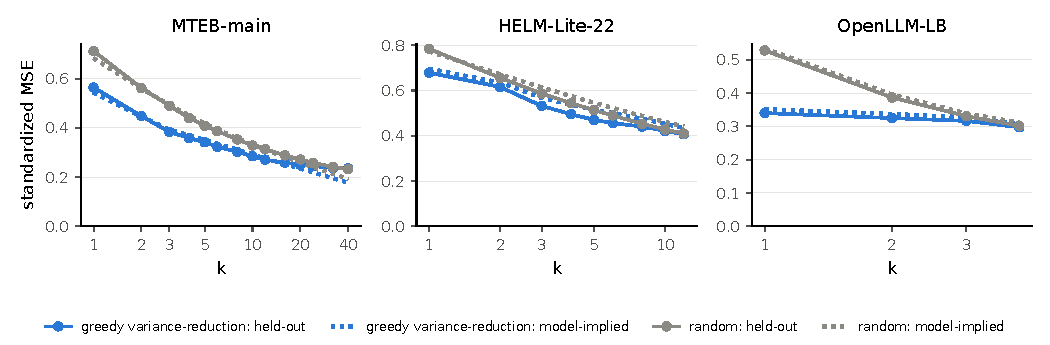
\includegraphics[width=\linewidth]{figs/calibration.pdf}
\caption{Model-implied expected MSE (dotted) vs.\ held-out MSE (solid) for greedy and random selection.}
\label{fig:calib}
\end{figure}

\begin{figure}[h]
\centering
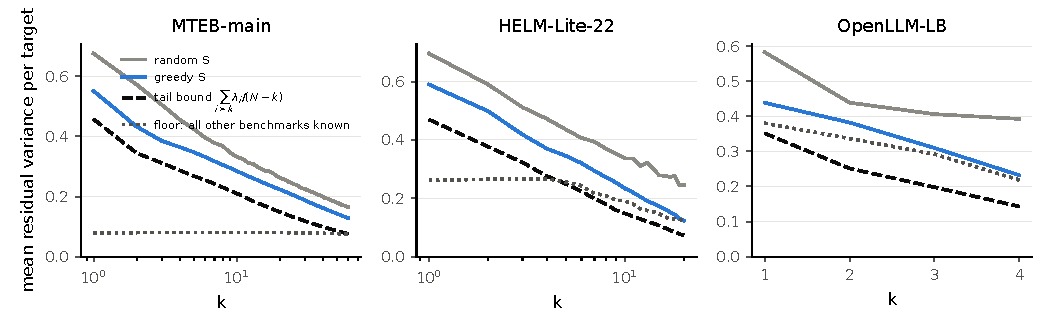
\includegraphics[width=\linewidth]{figs/spectral.pdf}
\caption{In-sample view on the full matrices (pairwise correlation matrix, light shrinkage): mean residual variance per remaining benchmark for random and greedy sets, the spectral tail bound of Prop.~\ref{prop:tail}, and the floor if all other benchmarks were known. Greedy sits between random and the bound.}
\label{fig:spectral}
\end{figure}

\paragraph{Aggregate error.} Mean absolute error (score points) of the \emph{average} of the held-out scores of a model (MTEB-main, \textsc{Gauss}, random splits; 95\% bootstrap CI): greedy 3.8 [3.5, 4.2] at $k=1$, 2.1 [1.9, 2.3] at 3, 1.7 [1.6, 1.9] at 5, 1.3 [1.2, 1.4] at 10, 1.1 [1.0, 1.2] at 20; random 6.2 [5.9, 6.5], 3.7 [3.5, 3.8], 2.7 [2.6, 2.8], 1.8 [1.7, 1.9], 1.3 [1.2, 1.4]; mean baseline 10.5. The RMSE per individual held-out benchmark is 11.0, 8.7, 8.0, 7.2, 6.9 (greedy) and 17.4 (baseline).

\paragraph{Ranking quality.} The per-benchmark Spearman correlation between predicted and actual scores across held-out models (MTEB-main, \textsc{Gauss}; average over benchmark$\times$fold pairs with $\ge8$ models) is 0.79/0.81/0.82 for greedy and 0.76/0.78/0.81 for random selection at $k=5/10/20$; MTEB-dense 0.77/0.78/0.79 vs.\ 0.73/0.77/0.79; HELM-Lite-22 0.71/0.72 vs.\ 0.68/0.74 at $k=5/10$. Models are therefore ranked well on any single benchmark with a handful of runs, and selection helps ranking less than it helps error.

\paragraph{Stability of the selected sets.} Running the greedy rule on each of the 15 training folds of the MTEB-main random splits (all 280 tasks as candidates, default shrinkage 0.05), the selected sets overlap only moderately: mean pairwise Jaccard similarity 0.23, 0.26, 0.26 at $k=5,10,20$ (a random set would give 0.01, 0.02, 0.04), because many tasks are near-substitutes. The most frequent first-ten picks are CyrillicTurkicLangClassification (13 of 15 folds), STS14 (12), TempReasonL2Fact (10), CQADupstackPhysicsRetrieval (10), AngryTweetsClassification (8) and BelebeleRetrieval (8). A practitioner should therefore treat the greedy list as one of many near-equivalent good subsets.

\paragraph{Number of models in the evaluation.} After requiring all budgets to be available for a cell, MTEB-main random splits use 189 models and 1,134 (model, fold, target-draw) cells, MTEB-main time-split 53 models; MTEB-eng 110 models; OpenLLM 4,496 (random) and 1,332 (temporal); HELM 91; LiveBench 158 in the first-3 budgets.
